

\chapter{Option pricing with transaction costs}\label{Chapter5}
%\blindtext
\minitoc% Creating an actual minitoc

\vspace{5em}

\section{Transaction costs models for the portfolio selection problem}
In the mathematical finance literature, the first application of stochastic optimal control theory to finance appears in the seminal paper \cite{Me69}.
This is the classical \emph{Merton optimal portfolio problem}, and is formulated as follows. An investor has a portfolio consisting of two assets, one ``risk free" $B$,
and the other ``risky" $S$. The assets in the portfolio have dynamics
\begin{equation}\label{Merton_problem1}
 \begin{cases}
 dB_t &=  rB_t dt \\
 dS_t &=  S_t \left( \mu dt + \sigma dW_t \right),
\end{cases}
\end{equation} 
with $\mu>r$ and $\sigma>0$. If we denote with $\mathcal{W}_t = B_t + S_t$  the wealth at time $t$, and with $\pi_t$ the fraction of wealth invested in the risky asset, such that
$S_t = \pi_t \mathcal{W}_t$ and $B_t = (1-\pi_t) \mathcal{W}_t$. The model also considers the investor consumption $\{c_t\}_{0 \leq t \leq T}$. 
The optimization problem can be formulated considering the utility function of the consumption and the terminal condition. It consists in maximizing the objective function
\begin{equation}
 J(x;\pi,c) = \E_x \biggl[ \int_0^{T} e^{-\beta t} \mathcal{U}(c_t) dt + g(T,\mathcal{W}_T) \biggr],
\end{equation}
where $\beta > 0$ and $\mathcal{U}: [0,\infty) \to \R$ is a concave and increasing utility function, such that $\mathcal{U}(0)=0$.
In the original article, the function $g$ is called \emph{bequest valuation function} and is assumed to be concave.
We indicate the initial portfolio state with $x = (B_0,S_0)$. 
The wealth $\mathcal{W}$ takes value in $\OO = (0,\infty)$ and has state dynamics
\begin{equation}
 d \mathcal{W}_t = (1-\pi_t) \mathcal{W}_t r dt + \pi_t \mathcal{W}_t (\mu dt + \sigma dW_t) - c(t)dt.
\end{equation}
The control $\alpha_t$ is a two dimensional vector $(\alpha^1_t,\alpha^2_t) = (\pi_t,c_t)$, with values in $A = \R \times [0,\infty)$. 
This is a finite horizon problem with an objective function of type (\ref{cost_functional})
and HJB equation as in (\ref{DPE}). 
Even if in this case the control space $A$ is not compact, the supremum in (\ref{DPE}) is attained, thanks to the concave structure of the problem.

Merton, using the utility $\mathcal{U}(c) = \frac{1}{\gamma} c^{\gamma}$ with $0<\gamma<1$ (of HARA type) obtained an explicit solution for the problem. In particular he found that 
the optimal control
\begin{equation}\label{Merton_policy}
  \pi^*_t = \frac{\mu-r}{(1-\gamma)\sigma^2}
\end{equation}
is a constant and does not depend on the state variables.  
This means that the optimal fraction of the risky and risk free assets in the portfolio is constant.
The line containing all the optimal points in the $(B,S)$-plane is the so called \textbf{Merton line}.

%In Chapter \ref{Chapter4} we have not considered infinite horizon control problems because they are not relevant for the thesis.
%The Merton optimal portfolio problem can be formulated as well in a finite time horizon setting, and removing the consumption rate. The objective function becomes
%\begin{equation}\label{Merton_problem2}
% J(t,x;\pi) = \E_{t,x} \biggl[ \mathcal{U}\biggl( \mathcal{W}^{\pi}(T) \biggr) \biggr] \quad \mbox{ for } \quad t \in [t_0,T].
%\end{equation}
%It turns out that the finite horizon solution is the same as the original infinite horizon Merton problem. The optimal policy is still given by formula (\ref{Merton_policy}).
%For the explicit derivation see for instance \cite{Pham}.

\noindent
The Merton portfolio selection problem is the first optimal portfolio problem solved by stochastic control theory methods. 
In \cite{Me71} the author extends the results to different utility functions.
All the successive models are generalizations of the Merton model, where by 
the word ``generalizations", we mean that under some particular choices of the parameters, the Merton problem is included in those models as a special case.
For what concerns this thesis, we review the main portfolio selection problems that have appeared in the literature, considering the presence of proportional transaction costs.
The first portfolio selection model with transaction costs and consumption was introduced by \cite{Co86} and then extended by \cite{DaNo90}. We refer to \cite{ShSo94}
for a viscosity solution approach to the same problem. 
Other important contributions are 
\cite{DaYi09}, \cite{Dai10}, \cite{LiuLo02}, \cite{LiuLo07}, \cite{BKR01}, \cite{OkSu01}, \cite{Kab16} where the last four articles use Lévy processes to model the stock dynamics. 
All the cited works are portfolio optimization models formulated as infinite horizon problems, and do not involve the pricing of the options.

Further assumptions are needed when the portfolio process is introduced for the purpose of pricing a derivative contract.
The main contributions on option pricing with transaction costs, using the \emph{indifference pricing} approach are
\cite{HoNe89} and \cite{DaPaZa93} (DPZ). The problem is formalized as a finite horizon singular stochastic control problem.
In this section we present the DPZ model, which is the building block of this thesis, and then extend it following the framework introduced by \cite{Kab16}, 
that consider the stock dynamics described by Lévy processes.



\subsection{Davis - Panas - Zariphopoulou (DPZ)}\label{DPZ_sec}

This is the market model with proportional transaction costs presented in \cite{DaPaZa93}. 
The authors consider a portfolio composed by one risk-free asset $B$ (bank account) paying a fixed interest rate $r > 0$ and a stock $S$. 
The symbol $Y$ denotes the number of shares of the stock $S$ that the investor holds. 
The state of the portfolio at time $t\in [t_0,T]$ is $(B^{\pi}_t,Y^{\pi}_t,S_t)$, and is the solution of the following the SDE:
\begin{equation}\label{DPZ_porfolio_dynamics}
 \begin{cases}
 dB^{\pi}_t &=  rB^{\pi}_t dt - (1+\theta_b)S_t dL_t + (1-\theta_s) S_t dM_t \\
 dY^{\pi}_t &=  dL_t - dM_t \\
 dS_t &=  S_t \left( \mu dt + \sigma dW_t \right).
\end{cases}
\end{equation} 
for a particular strategy $\{\pi_t\}_{t \in [t_0,T]} := \{(L_t,M_t)\}_{t \in [t_0,T]}$.
The parameters $\theta_b$, $\theta_s \geq 0$ are the proportional transaction costs when buying and selling respectively.
This portfolio equation is a generalization of the portfolio in the Merton problem (\ref{Merton_problem1}), 
where there is a new state variable $Y$ and the action of the controls is represented with a different approach.
The control process $\{\pi_t\}_{t \in [t_0,T]} := \{(L_t,M_t)\}_{t \in [t_0,T]}$ represents the trading strategy and indicates the 
cumulative number of shares bought and sold respectively in $[t_0,T]$.
The strategy $\pi_t$ is a cádlág, $\mathcal{F}_t$-progressively measurable, nondecreasing process with bounded variation in every finite time interval and such that
$ \pi_{t_0^-} = ( L_{t_0^-} , M_{t_0^-} ) = (0,0) $, allowing for an initial transaction at $t_0$.\\
In the discontinuity points of $L_t$ and $M_t$ we indicate the process variation with $\Delta L_t= L_{t}-L_{t^-}$ and $\Delta M_t= M_{t}-M_{t^-}$.

% In order to understand better the mechanism, let us make a recap:
% \begin{itemize}
%  \item Variation in the number of shares:
%  $$\Delta Y^{\pi}_t =  \underbrace{\Delta L_t}_{\mbox{shares bought}} - \underbrace{\Delta M_t}_{\mbox{shares sold}} $$
%  \item Variation in the bank account:
%  $$ \Delta B^{\pi}_t =  - \underbrace{(1+\theta_b)S_t}_{\mbox{adjusted price}} \Delta L_t + \underbrace{(1-\theta_s) S_t}_{\mbox{adjusted price}} \Delta M_t $$
% \end{itemize}
% we can identify this problem as a singular stochastic control problem as described in Chapter \ref{singular_control}.


\begin{Definition}
We define the \textbf{cash value} function $c(y,s)$ as the value in cash when the shares in the portfolio are liquidated, i.e.  
long positions are sold and short positions are covered.
\begin{equation}\label{cost_function}
c(y,s) = \begin{cases} 
(1+\theta_b)ys, & \mbox{if } y\leq 0 \\ 
(1-\theta_s)ys, & \mbox{if } y>0 . 
\end{cases} 
\end{equation} 
\end{Definition}
\begin{Definition}
For $t\in [t_0,T]$, we define the \textbf{total wealth} process:
\begin{equation}\label{wealth_process}
 \mathcal{W}^{\pi}_t = B^{\pi}_t + c(Y^{\pi}_t,S_t).
\end{equation} 
\end{Definition}
We say that a portfolio is solvent if the portfolio's wealth $\mathcal{W}_t$ is greater than a fixed constant $-C$, with 
$C\geq0$ that may depend on the initial wealth and on the parameters in (\ref{DPZ_porfolio_dynamics}). 
This constant may be interpreted as the \emph{credit availability} of the investor.
\begin{Definition}
We define the \textbf{solvency region}:
\begin{equation}\label{solvency_region}
 \mathcal{S} := \biggl\{ (b,y,s) \in \R \times \R \times \R^+ : b + c(y,s) > -C  \biggr\}.
\end{equation} 
\end{Definition}
\begin{Definition}\label{admissible_strategies1}
The set of \textbf{admissible trading strategies} $\Pi(t_0,b,y,s)$, is defined   
as the set of all right-continuous, nondecreasing, $\mathcal{F}_t$-progressively measurable processes  
$\{\pi_t\}_{t \in [t_0,T]}$, such that $(B^\pi_t,Y^\pi_t,S_t)$ is a solution of (\ref{DPZ_porfolio_dynamics}) with initial values $(B^\pi_{t_0} = b, Y^\pi_{t_0} = y, S_{t_0} = s)$, 
and 
\begin{equation}
 \mathcal{W}^{\pi}_t \in \mathcal{S}
\end{equation}
for $t \in [t_0,T]$ almost surely.
\end{Definition}

\begin{Remark}
In the first problem formulation of \cite{HoNe89}, the authors 
consider a portfolio starting with zero total wealth. 
The writer (or buyer) of the option creates a portfolio at time $t_0$ with the purpose of hedging the option.
It is reasonable to assume that no shares of the underlying stock are contained in the portfolio at time $t_0$. 
In the numerical computations of Chapter \ref{Chapter6}, we will consider portfolios with zero initial shares and initial cash amount $B_0$. 
The model is able to compute option prices for an investor with any initial number $Y_0$ of shares if needed.
\end{Remark}



\subsubsection{Utility maximization}


Let us assume an investor builds a portfolio with cash, shares of a stock and in addition he sells or purchases a 
European call option written on the same stock, with strike price $K$ and expiration date $T$.\\
From now on, we introduce the superscripts $w$, $b$ and $0$ to indicate the writer, buyer and zero-option portfolios respectively.
In the zero-option portfolio, the wealth process $\{\mathcal{W}^{0; \pi}_t\}_{t \in [t_0,T]}$ corresponds to (\ref{wealth_process}).
\begin{Definition}
For $t \in [t_0,T]$, we define the wealth processes for the writer:
  \begin{align}\label{wealth_writer}
   \mathcal{W}^{w; \pi}_t := & \; B^{\pi}_t + c(Y^{\pi}_t,S_t) \mathbbm{1}_{\{t < T\}} \\ \nonumber
   & + c(Y^{\pi}_t,S_t) \mathbbm{1}_{\{t = T,\, S_t(1+ \theta_b ) \leq K\}}
   + \biggl( c\bigl( Y^{\pi}_t-1,S_t \bigr) + K \biggr) \mathbbm{1}_{\{t=T,\, S_t(1+ \theta_b ) > K \}}
  \end{align}
 and the buyer:
  \begin{align}\label{wealth_buyer}
   \mathcal{W}^{b; \pi}_t := & \; B^{\pi}_t + c(Y^{\pi}_t,S_t) \mathbbm{1}_{\{t < T\}} \\ \nonumber
   & + c(Y^{\pi}_t,S_t) \mathbbm{1}_{\{t = T,\, S_t(1+ \theta_b ) \leq K\}}
   + \biggl( c\bigl( Y^{\pi}_t+1,S_t \bigr) - K \biggr) \mathbbm{1}_{\{t=T,\, S_t(1+ \theta_b ) > K \}}.
  \end{align}
\end{Definition}

\begin{figure}[t!]
 \centering
 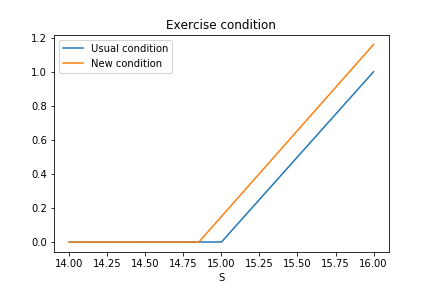
\includegraphics[scale=0.5]{payoff_comparison.png}
 % payoff_comparison.png: 0x0 pixel, 300dpi, 0.00x0.00 cm, bb=
 \caption{Comparison of payoffs of an European Call option with strike $K=15$, in a market with zero costs and in a market with $\theta_b=0.01$.}
 \label{fig:payoff_comparison}
\end{figure}
In the case the option is exercised, $S_T(1+ \theta_b ) > K$, the buyer pays to the writer the strike value $K$ in cash, 
and the writer delivers one share to the buyer.
In a market with transaction costs the real value (in cash) of a share incorporates the transaction costs. 
Therefore the buyer does not exercise when $S_T > K$, but when $S_T(1+ \theta_b ) > K$. 
In figure \ref{fig:payoff_comparison} there is a comparison between the payoff in a market with zero costs (such as in the Black-Scholes model) and a market with 
transaction costs.

The objective of the investor is to maximize the expected utility of the wealth at terminal time $T$ over all the admissible
strategies. This expectation is conditioned on the current value of cash, number of shares and value of the
stock.
The sets of trading strategies corresponding to each of the three portfolios, is obtained by using the respective wealth process inside Definition [\ref{admissible_strategies1}]. 

\begin{Definition}
 The \textbf{value function} of the maximization problem for $j=w,b,0$ is defined as:
\begin{align}\label{max_probl0}
V^j(t,b,y,s) := \sup_{\pi \in \Pi^j(t,b,y,s)} \; & \E_{t,b,y,s}\biggl[ 
            \mathcal{U}(\mathcal{W}^{j; \pi}_T) \biggr],             
\end{align}
where $\mathcal{U}: \R \to \R$ is a concave increasing utility function such that $\mathcal{U}(0)=0$.
\end{Definition}

The writer (buyer) option price is defined as the amount of cash to add (subtract) to the bank account, 
such that the maximal expected utility of wealth of the writer (buyer) is the same he could get with 
the zero-option portfolio.
\begin{Definition}
The writer price is the value $p^w>0$ such that 
 \begin{equation}\label{writer}
  V^0(t,b,y,s) = V^w(t,b+p^w,y,s),
 \end{equation}
 and the buyer price is the value $p^b>0$ such that
 \begin{equation}\label{buyer}
  V^0(t,b,y,s) = V^b(t,b-p^b,y,s).
 \end{equation}
\end{Definition}


\subsubsection{HJB Equation}\label{subsec_HJB}

According to the theory of stochastic optimal control presented in Chapter \ref{Chapter4},  
we can identify the DPZ model within the class of singular control problems described in Section (\ref{singular_control}).
Let us re-write the state equation (\ref{DPZ_porfolio_dynamics}) for $X^{\pi}_t = (B^{\pi}_t,Y^{\pi}_t,S_t)$ in the matrix form 
\begin{align}\label{DPZ_porfolio_dynamicsM}
d X^{\pi}_t
=& 
 d \left(
\begin{array}{l}
B^{\pi}_t\\
Y^{\pi}_t\\
S_t
\end{array} \right) \\ \nonumber
  =&  \left( \begin{array}{l}
r B^{\pi}_t\\
0\\
\mu S_{t}
\end{array} \right)
dt +  \left( \begin{array}{l}
0\\
0\\
\sigma S_{t}
\end{array} \right) dW_t \\ \nonumber
&+ \underbrace{\left( \begin{array}{cc}
-S_{t}(1+\sigma_b) & S_{t}(1-\sigma_s) \\
1 & -1 \\
0 & 0
\end{array} \right)}_{\kappa(t,X_t)}
\underbrace{\left( \begin{array}{l}
dL_t \\
dM_t 
\end{array} \right)}_{d\xi_t},
\end{align}
which can be easily identified with the general equation (\ref{singular_SDE}).
The state $X^{\pi}_t$ takes values in $\OO$ corresponding to the solvency region $\SI$.
The value function (\ref{max_probl0}) has a cost functional as in (\ref{singular_cost_functional}) with $f$ and $h$ equal to zero. 


According to singular control theory, the HJB equation of a singular control problem is a variational inequality. Here we can obtain the HJB equation of this problem 
from the general equation (\ref{variational_inequality}). We omit the subscript of $V^j$ when the discussion refers to all the three problems. 
Let us indicate $x = (b,y,s)$, then
\begin{itemize}
 \item $ D_x V(t,x) = \left( \frac{\partial V(t,b,y,s)}{\partial b}, \frac{\partial V(t,b,y,s)}{\partial y}, \frac{\partial V(t,b,y,s)}{\partial s} \right) $
 \item $H(t,x,p) = \sup_{a \in \hat K} \bigl( p \cdot \kappa(t,x) \cdot a  \bigr) \quad \mbox{ and define } 
        \quad \hat K = \left( \begin{array}{c}
			   1 \\
			   0
                          \end{array} \right) \bigcup \left( \begin{array}{c}
			   0 \\
			   1
                          \end{array}
  \right)$ 
 \item $H \bigl(t,x, D_x V(t,x) \bigr) = \max \biggl\{ \frac{\partial V}{\partial y}-(1+\theta_b) s \frac{\partial V}{\partial b} ,
 -\bigl( \frac{\partial V}{\partial y} -(1-\theta_s)s \frac{\partial V}{\partial b} \bigr) \biggr\} $
\end{itemize}
The resulting HJB equation is
\begin{align}\label{DPZ_HJB}
& \max \; \biggl\{ \; \frac{\partial V}{\partial t} + rb\frac{\partial V}{\partial b} 
+ \mu s \frac{\partial V}{\partial s} + \frac{1}{2}\sigma^2 s^2 \frac{\partial^2 V}{\partial s^2}, \\ \nonumber
& \;  \frac{\partial V}{\partial y}-(1+\theta_b) s \frac{\partial V}{\partial b} \; 
, \; -\biggl(\frac{\partial V}{\partial y}-(1-\theta_s)s \frac{\partial V}{\partial b} \biggr) \biggr\} = 0, 
\end{align}
for $(t,b,y,s) \in [t_0,T] \times \SI$.
The terminal conditions for the three portfolio problems $j=0,w,b$ are:
\begin{equation}\label{terminal_conditions}
V^j(T,b,y,s) = \mathcal{U}\bigl( w^j(b,y,s) \bigr) \hspace{1em} \mbox{ for } \hspace{1em} (b,y,s) \in \mathcal{S}^j 
\end{equation}
with
  \begin{equation*}
   w^0(b,y,s) =  b + c(y,s).
  \end{equation*}
  \begin{equation*}
   w^w(b,y,s) =  b + c(y,s) \mathbbm{1}_{\{ s(1+\theta_b) \leq K\}} +
  \biggl( c\bigl( y-1,s \bigr) + K \biggr) \mathbbm{1}_{\{s(1+\theta_b)>K\}}.
  \end{equation*}
  \begin{equation*}
   w^b(b,y,s) = b + c(y,s) \mathbbm{1}_{\{ s(1+\theta_b) \leq K\}} +
  \biggl( c\bigl( y+1,s \bigr) - K \biggr) \mathbbm{1}_{\{s(1+\theta_b)>K\}}.
  \end{equation*}

\noindent
The variational inequality (\ref{DPZ_HJB}) says that the maximum of three operators is equal to zero.
This feature can be interpreted better if we consider the state space divided into three different regions: the \textbf{Buy}, the \textbf{Sell}
and the \textbf{No Transaction} (NT) regions.
\begin{itemize}
 \item \textbf{Buy}
  \begin{equation*}
   \begin{cases}
     & \frac{\partial V}{\partial t} + rb\frac{\partial V}{\partial b} + \mu s \frac{\partial V}{\partial s} + \frac{1}{2}\sigma^2 s^2 \frac{\partial^2 V}{\partial s^2} \leq 0\\ 
     & \frac{\partial V}{\partial y}-(1+\theta_b) s \frac{\partial V}{\partial b} = 0 \\
     & -\biggl(\frac{\partial V}{\partial y}-(1-\theta_s)s \frac{\partial V}{\partial b} \biggr) \leq 0.
   \end{cases}
  \end{equation*}
 \item \textbf{Sell}
  \begin{equation*}
   \begin{cases}
     & \frac{\partial V}{\partial t} + rb\frac{\partial V}{\partial b} + \mu s \frac{\partial V}{\partial s} + \frac{1}{2}\sigma^2 s^2 \frac{\partial^2 V}{\partial s^2} \leq 0 \\ 
     & \frac{\partial V}{\partial y}-(1+\theta_b) s \frac{\partial V}{\partial b} \leq 0 \\
     & -\biggl(\frac{\partial V}{\partial y}-(1-\theta_s)s \frac{\partial V}{\partial b} \biggr) = 0.
   \end{cases}
  \end{equation*}
 \item \textbf{No Transaction}
  \begin{equation*}
   \begin{cases}
     & \frac{\partial V}{\partial t} + rb\frac{\partial V}{\partial b} + \mu s \frac{\partial V}{\partial s} + \frac{1}{2}\sigma^2 s^2 \frac{\partial^2 V}{\partial s^2} = 0 \\ 
     & \frac{\partial V}{\partial y}-(1+\theta_b) s \frac{\partial V}{\partial b} \leq 0 \\
     & -\biggl(\frac{\partial V}{\partial y}-(1-\theta_s)s \frac{\partial V}{\partial b} \biggr) \leq 0.
   \end{cases}
  \end{equation*}
\end{itemize}
The optimization problem is a free boundary problem, and its solution consists of finding the value function $V$ and the 
optimal boundaries that divide the three regions.
We assume that the Buy and Sell regions are separated by the NT region. This assumption is reasonable since buying and selling a share at the same time just decreases the 
total wealth (because of the transaction costs) and therefore makes no sense. 

The free boundaries of the NT region completely characterize the investor's trading strategy.
The optimal strategy consists in keeping the portfolio process inside the NT region. 
If the portfolio exits the NT region, the optimal strategy is to trade in order to bring it back to the NT region.

In the Buy and Sell regions the value functions is constant along the directions of the trades.
We get respectively:
\begin{itemize}
 \item[Buy]: \hspace{2em} $V(t,b,y,s) = V(t,b-s(1+\theta_b)\Delta L_t,y+\Delta L_t,s).$
 \item[Sell]: \hspace{2em} $ V(t,b,y,s) = V(t,b+s(1-\theta_s)\Delta M_t,y-\Delta M_t,s).$
\end{itemize}
where $\Delta L_t$ and $\Delta M_t$ are the number of shares respectively bought or sold in the trade.
%In the NT region the portfolio evolves according to the portfolio equation (\ref{DPZ_porfolio_dynamics}), with $dL=dM=0$.
%It means that the number of shares remains constant as long as the portfolio stays in the NT region.





\subsection{DPZ with jumps}\label{DPZ_j_sec}


The purpose of this thesis is to extend the DPZ model in order to include jumps in the stock dynamics. 
Following the framework of \cite{Kab16} let us introduce a market model with proportional transaction costs 
that consider an exponential Lévy process for the stock dynamics, as in \ref{exp_sde2}.
The state of the portfolio at time $t\in [t_0,T]$ is $(B^{\pi}_t,Y^{\pi}_t,S_t)$ and evolves following the SDE:
\begin{equation}\label{porfolio_dynamics}
 \begin{cases}
 dB^{\pi}_t &=  rB^{\pi}_t dt - (1+\theta_b)S_{t^-} dL_t + (1-\theta_s) S_{t^-} dM_t \\
 dY^{\pi}_t &=  dL_t - dM_t \\
 dS_t &=  S_{t^-} \left( \mu dt + \sigma dW_t + \int_{\R} (e^z-1) \tilde N(dt,dz) \right).
\end{cases}
\end{equation}
The strategy $\{\pi_t\}_{t \in [t_0,T]}$ is a cádlág, \textbf{predictable}, nondecreasing process with bounded variation, such that
$ \pi_{t_0^-} = \bigl ( L_{t_0^-} , M_{t_0^-} \bigr ) = (0,0)$.
Under these assumptions the portfolio process 
$\bigl \{(B^{\pi}_t,Y^{\pi}_t,S_t)\bigr \}_{t \in [t_0,T]}$ is cádlág.

If at time $t$ there is an unpredictable jump in the stock price $\Delta S_t = S_t - S_{t^-}$, a possible transaction should happen immediately after the jump.
The control process $\{\pi_t\}_{t \in [t_0,T]}$ is assumed to be predictable, i.e. measurable with respect to the left-continuous filtration generated by $\{S_{t^-}\}_{t \in [t_0,T]}$.
Therefore, a jump in the price and a jump in the control cannot occur simultaneously, almost surely. 
A deeper digression on this topic can be found in Section 2 of \cite{Kab16}.   
If the investor at time $t$ observes a jump in the price and decides to rebalance his portfolio, he will trade at some time $u>t$ at the price $S_{u^-}$. 
Under this framework, as explained in \cite{Kab16}, the optimal strategy cannot exist. 

The definitions of cash value (\ref{cost_function}), of total wealth (\ref{wealth_process}), (\ref{wealth_buyer}), (\ref{wealth_writer}) and the solvency regions
(\ref{solvency_region}) are kept the same. The set of admissible trading strategy will be changed.

Since the underlying stock follows a process with jumps, it is not guaranteed that the portfolio stays
solvent for all $t \in [t_0,T]$. When holding short positions, it is possible that a sudden increase in the stock price 
cause the total wealth to jump out of the solvency region. 
The same can happen with a downward jump when the investor is long in stocks and negative in cash. 
The immediate decrease of the stock's price makes him unable to pay the debts.
If the investor goes bankrupt, there are no trading strategies to save him.
\begin{Definition}
The first \textbf{exit time} from the solvency region is defined as:
\begin{equation}\label{exit_time}
 \tau := \inf \bigl\{ t \in [t_0,T] : \mathcal{W}^{\pi}_t \not\in \SI \bigr\}.
\end{equation} 
\end{Definition}
\begin{Definition}\label{set_trad_strat}
The set of \textbf{admissible trading strategies} $\Pi(t_0,b,y,s)$   
is the set of all cádlág, nondecreasing, predictable, bounded variation processes $\{\pi_t\}_{t \in [t_0,T]}$
such that $(B^\pi_t,Y^\pi_t,S_t)$ is a solution of (\ref{porfolio_dynamics}) with initial values $(B^\pi_{t_0} = b, Y^\pi_{t_0} = y, S_{t_0} = s)$ and such that
$\mathcal{W}^{\pi}_t \in \SI$ almost surely for all $t\in [t_0,\tau)$, and $\pi_t = \pi_{\tau}$ for all $t \geq \tau$.  
\end{Definition}

The objective of the investor is to maximize the expected utility of the wealth at $\tau^j \wedge T$ over all the admissible
strategies. This expectation is conditioned on the current value of cash, number of shares and value of the
stock.
\begin{Definition}
 The \textbf{value function} of the maximization problem for $j=w,b,0$ is defined as:
\begin{align}\label{max_probl1}
V^j(t,b,y,s) := \sup_{\pi \in \Pi^j(t,b,y,s)} \; & \E_{t,b,y,s}\biggl[ 
            \mathcal{U}(\mathcal{W}^{j; \pi}_T) \; \mathbbm{1}_{\{\tau^j > T\}} \\ \nonumber
             &+ e^{ \beta (T-\tau^j)} \mathcal{U}( \mathcal{W}^{j; \pi}_{\tau^j} ) \; 
             \mathbbm{1}_{\{\tau^j \leq T\}}\biggr],             
\end{align}
where $\mathcal{U}: \R \to \R$ is a concave increasing utility function such that $\mathcal{U}(0)=0$, and $\beta \geq 0$.
\end{Definition}

The HJB equation associated to this stochastic control problem is obtained following the same steps we used to derive (\ref{DPZ_HJB}). The infinitesimal generator of the price 
dynamics has the 
form (\ref{inf_gen_exp_levy}) for exponential Lévy processes. The HJB variational inequality is
\begin{align}\label{HJB1}
& \max \; \biggl\{ \; \frac{\partial V^j}{\partial t} + rb\frac{\partial V^j}{\partial b} 
+ \mu s \frac{\partial V^j}{\partial s} + \frac{1}{2}\sigma^2 s^2 \frac{\partial^2 V^j}{\partial s^2} \\ \nonumber
&+ \int_\mathbb{R}
\biggl[ V^j(t,b,y,se^z) - V^j(t,b,y,s) - s(e^z-1)\frac{\partial V^j}{\partial s} \biggr] \nu(dz) \;,\\ \nonumber
& \;  \frac{\partial V^j}{\partial y}-(1+\theta_b) s \frac{\partial V^j}{\partial b} \; 
, \; -\biggl(\frac{\partial V^j}{\partial y}-(1-\theta_s)s \frac{\partial V^j}{\partial b} \biggr) \biggr\} = 0, 
 \end{align}
for $(t,b,y,s) \in [t_0,T) \times \SI^j$ and $j=0,w,b$.   
The terminal boundary conditions are given by Eq. (\ref{terminal_conditions}).
Since this HJB equation is a PIDE,
the non-local integral operator implies to 
define the lateral conditions not only on the boundary
of the solvency region, but also beyond:
\begin{equation}\label{lat_bound}
V^j(t,b,y,s) = e^{ \beta (T-t)} \mathcal{U}\bigl( b + c(y,s)\bigr) \hspace{1em} \mbox{ for } \hspace{1em} 
t \in [t_0,T) , \hspace{0.5em} (b,y,s) \not \in \mathcal{S}, \hspace{1em} j=0,w,b. 
\end{equation}


\subsection{Variable reduction}\label{variable_reduction}


In the DPZ model introduced in Section \ref{DPZ_sec}, the portfolio is solvent for every
$t \in [t_0,T]$ and it is always possible to calculate the utility 
of the wealth at the terminal time $\mathcal{U}(\mathcal{W}^{\pi}_T)$.
In the extended model of Section \ref{DPZ_j_sec} the stock process can jump, and in presence of short positions the portfolio can go bankrupt at any time before the maturity $T$. 

With the intention of simplifying the maximization problem (\ref{max_probl1}) and reducing the number of variables, 
%we restrict our attention to the subset of solvent paths. 
we restrict our attention to the case of no bankruptcy.
A possible idea is to consider a positive initial wealth, and define the restricted set of admissible strategies as the set of $\{\pi_t\}_{t \in [t_0,T]}$ such that 
$B^{\pi}_t \geq 0$ and $Y^{\pi}_t \geq 0$ for all $t\in [t_0,T]$ (see \cite{Benth02}).
However, in order to implement a hedging strategy, we are interested in portfolios containing short positions as well.
So, we can assume that the investor has a very large credit availability $C$ in the sense that
\begin{equation}\label{P_tau}
 \PP(\tau > T) \underset{C\to \infty}{\approx} 1.
\end{equation}
In practical terms, we ignore the possibility of default. The solvency region becomes $\mathcal{S} = \R^2 \times \R^{+}$ and no lateral boundary conditions are imposed.

As in \cite{DaPaZa93}, for $\gamma>0$, we consider the exponential utility function
\begin{equation}\label{exp_util}
 \mathcal{U}(x) := 1- e^{-\gamma x}.
\end{equation}
Thanks to (\ref{P_tau}) and (\ref{exp_util}) we can remove $\{B^{\pi}_t\}_{t \in [t_0,T]}$ from the state dynamics.
By solving (\ref{porfolio_dynamics}) we get
\begin{equation}\label{BT}
B^{\pi}_T =  \frac{B^{\pi}_{t}}{\delta(t,T)} - \int_{t}^T
(1+\theta_b)\frac{S_u}{\delta(u,T)} dL_u + \int_{t}^T
 (1-\theta_s) \frac{S_u}{\delta(u,T)} dM_u 
\end{equation}
where $\delta(u,T) = e^{-r(T-u)}$.
Using together (\ref{P_tau}), (\ref{exp_util}) and (\ref{BT}), and the wealth processes (\ref{wealth_process}),(\ref{wealth_writer}),(\ref{wealth_buyer}), 
we obtain for $B^\pi_{t} = b$, $Y^\pi_{t} = y$, $S_{t} = s$ and $j=0,w,b$:
\begin{align}\label{var_reduct}
   V^j(t,b,y,s) = \sup_{\pi} \; \E_{t,b,y,s}\biggl[  1- e^{-\gamma \mathcal{W}^j(T) } \biggr]  % \\ \nonumber 
	     = 1- e^{-\gamma \frac{b}{\delta(t,T)}} Q^j(t,y,s),
\end{align} 
where
\begin{align}\label{minimization}
Q^j(t,y,s) = \inf_{\pi} \; \mathbb{E}_{t,y,s}\biggl[ \; &
	     e^{-\gamma \bigl[ -\int_{t}^T (1+\theta_b) \frac{S_u}{\delta(u,T)} dL_u +
	     \int_{t}^T (1-\theta_s) \frac{S_u}{\delta(u,T)} dM_u \bigr] } \, \\ \nonumber 
	     & \times H^j(Y^{\pi}_T,S_T) \bigg]  
\end{align}
is our new minimization problem.
The exponential term inside the expectation can be considered as a discount factor, and the second term 
$H^j(y,s) = Q^j(T,y,s)$ is the terminal payoff:
\begin{itemize}
 \item No option:
 \begin{equation}\label{terminal_c}
  H^0(y,s) = e^{-\gamma \, c(y,s)}.
 \end{equation}
 \item Writer:
  \begin{equation}\label{terminal_w}
  H^w(y,s) = e^{-\gamma \bigl[ c(y,s)\mathbbm{1}_{\{s(1+\theta_b) \leq K\}} + 
 \bigl( c( y-1,s) + K \bigr) \mathbbm{1}_{\{s(1+\theta_b)>K\}} \bigr] }.
 \end{equation}
 \item Buyer:
  \begin{equation}\label{terminal_b}
  H^b(y,s) = e^{-\gamma \bigl[ c(y,s)\mathbbm{1}_{\{s(1+\theta_b) \leq K\}} + 
 \bigl( c( y+1,s) - K \bigr) \mathbbm{1}_{\{s(1+\theta_b)>K\}} \bigr] }.
 \end{equation}
\end{itemize}
Using conditions (\ref{writer}), (\ref{buyer}) together with (\ref{var_reduct}), we obtain the explicit formulas for the option prices:
\begin{equation}\label{opt_w}
 p^w(t_0,y,s) = \frac{\delta(t_0,T)}{\gamma} \log \biggl( \frac{Q^w(t_0,y,s)}{Q^0(t_0,y,s)} \biggr),
\end{equation}
\begin{equation}\label{opt_b}
 p^b(t_0,y,s) = \frac{\delta(t_0,T)}{\gamma} \log \biggl( \frac{Q^0(t_0,y,s)}{Q^b(t_0,y,s)} \biggr).
\end{equation}

Since $Q^j(t,y,s)$ is independent on $b$, let us write
$ Q^j(t,y,s) := 1 - V^j(t,0,y,s)$.
It is convenient to pass to the log-variable $x = \log(s)$, such that
\begin{equation}\label{log_var}
s \frac{\partial}{\partial s} = \frac{\partial}{\partial x}, \hspace{2em} 
s^2 \frac{\partial^2}{\partial s^2} = \frac{\partial^2}{\partial x^2} - \frac{\partial}{\partial x} . 
\end{equation}
For $j=0,w,b$, the HJB Eq. (\ref{HJB1}) becomes:
\begin{align}\label{HJB2}
& \min \; \biggl\{ \; \frac{\partial Q^j}{\partial t} + (\mu-\frac{1}{2}\sigma^2) \frac{\partial Q^j}{\partial x}
+ \frac{1}{2}\sigma^2 \frac{\partial^2 Q^j}{\partial x^2} \\ \nonumber
&+ \int_\mathbb{R}
\biggl[ Q^j(t,y,x+z) - Q^j(t,y,x) - (e^z-1)\frac{\partial Q^j}{\partial x} \biggr] \nu(dz) \;,  \\ \nonumber
& \; \frac{\partial Q^j}{\partial y} +(1+\theta_b) e^x \frac{\gamma}{\delta(t,T)}Q^j \; , 
\; -\biggl( \frac{\partial Q^j}{\partial y}+(1-\theta_s)e^x \frac{\gamma}{\delta(t,T)} Q^j 
\biggr) \biggr\} = 0. 
 \end{align}
% This equation is well defined for $Q^j \in C^{1,1,2}\bigl( (t_0,T) \times \R^2\bigr) \bigcap C_2\bigl( [t_0,T] \times \R^2 \bigr) $. 








\section{Existence of viscosity solution}

The general fact that value functions of control problems can be characterized as
viscosity solutions of certain partial differential equations is a direct consequence of the dynamic
programming principle. For singular control problems, however, the classical approach of \cite{PLL83}
fails because the state process may jump due to the singular control and it needs thus not stay
in a small ball\footnote{For processes of type (\ref{singular_SDE}) it is not possible to apply the theorem (\ref{stochastic_theorem}).} 
for a small $\Delta t$.
This problem can be circumvented by relying on the
existence of the optimal control, as done in \cite{DaPaZa93}. However, in our proof we will not assume the existence of the optimal control, which  
in this framework does not exist.
We will assume that the \textbf{DPP} for the singular control problem (\ref{porfolio_dynamics}), (\ref{max_probl1}) holds, and that the value function  
is continuous. We refer to sections 4 and 9 of \cite{Kab16} for the proofs of these statements. 

In this section we prove that the value function (\ref{max_probl1}), can be interpreted 
as the viscosity solution of the HJB equation (\ref{HJB1}).
The proof follows the approach in \cite{OkSu01}.

Let us call $\tau_{\SI}$ the first exit time from $\SI$.
Since the stock dynamics is stochastically continuous and (by definition) the control process $\pi$ cannot be the cause of bankruptcy,
we can exclude an immediate jump out of the solvency region, i.e. $t_0 \not = \tau_{\SI}$.

We have to interpret the HJB equation (\ref{HJB1}) with boundary conditions (\ref{lat_bound}) and (\ref{terminal_conditions}) 
as a parabolic problem of the type (\ref{parabolic_PIDE}). 
We use the dummy variable $x = (b,y,s)$ to indicate a point in $\R^2\times \R^+$. In order to satisfy the parabolic conditions we reformulate the HJB as 
\begin{align}\label{HJB22}
& \min \; \biggl\{ - \biggl( \; \frac{\partial V}{\partial t} + rb\frac{\partial V}{\partial b} 
+ \mu s \frac{\partial V}{\partial s} + \frac{1}{2}\sigma^2 s^2 \frac{\partial^2 V}{\partial s^2} \\ \nonumber
&+ \int_\mathbb{R}
\biggl[ V(t,b,y,se^z) - V(t,b,y,s) - s(e^z-1)\frac{\partial V}{\partial s} \biggr] \nu(dz) \; \biggr) ,\\ \nonumber
& \; - \biggl( \frac{\partial V}{\partial y}-(1+\theta_b) s \frac{\partial V}{\partial b} \biggr) \; 
, \; + \biggl(\frac{\partial V}{\partial y}-(1-\theta_s)s \frac{\partial V}{\partial b} \biggr) \biggr\} = 0. 
\end{align}
We indicate this function with
$ F(t,x,V,D_t V,D_{x} V,D_{xx}V,\I(t,x,V)) = 0$ in the domain $(t,x) \in [t_0,T) \times \SI$.
To simplify the notation, let us introduce the integro-differential infinitesimal generator:
\begin{align*}
 \LL V(t,x) &:= -\biggl( \frac{\partial V}{\partial t}(t,x) + rb\frac{\partial V}{\partial b}(t,x) 
  + \mu s \frac{\partial V}{\partial s}(t,x) + \frac{1}{2}\sigma^2 s^2 \frac{\partial^2V}{\partial s^2}(t,x)\biggr) \\
  &- \int_{\R}
\biggl[ V(t,b,y,se^z) - V(t,b,y,s) - s(e^z-1)\frac{\partial V}{\partial s} \biggr] \nu(dz),
\end{align*}
such that the equation (\ref{HJB22}) has the form
\begin{equation}\label{qvi_min}
  \min \; \biggl\{ \; \LL V(t,x),
  \, -(V_y-(1+\theta_b)sV_b) \, , \; V_y-(1-\theta_s)s V_b \biggr\} = 0.
\end{equation}
In order to prove that $V(t,x)$ is a viscosity solution we need to verify both the subsolution and supersolution properties.



\subsection{Subsolution}

In this section we prove that the value function can be interpreted as a viscosity subsolution of the HJB equation associated to the maximization problem. 
We enunciate the following theorem:
\begin{Theorem}\label{subsolution_th}
 The value function of the maximization problem (\ref{max_probl1}), is a viscosity subsolution of the Eq. (\ref{qvi_min}).
\end{Theorem}
\begin{proof}
Let us consider a test function $ \phi \in C^2([t_0,T] \times \R^2\times \R^+) \bigcap \mathcal{C}_2([t_0,T] \times \R^2\times \R^+)$ such that 
$(\bar t,\bar x) \in [t_0,T] \times \SI$ is a maximum point for $V-\phi$:
\begin{equation}
 V(\bar t,\bar x) - \phi(\bar t,\bar x) \geq V(t,x) - \phi(t, x) \hspace{2em} \forall (t,x) \in [t_0,T] \times \SI
\end{equation}
and we assume without loss of generality that:
\begin{equation}\label{max_point}
V(\bar t,\bar x) = \phi(\bar t,\bar x)  
\end{equation}
so we can write:
\begin{equation}\label{max_point2}
V(t,x) \leq \phi(t, x) 
\end{equation}
We want to prove that
$$ F(\bar t,\bar x,V(\bar t, \bar x),D_t \phi(\bar t, \bar x),D_x \phi(\bar t, \bar x),D_{xx}\phi(\bar t, \bar x),
\I(\bar t, \bar x,\phi(\bar t, \bar x))) \leq 0  $$
\textbf{Reductio ad absurdum:}\\
Let us assume that 
$$F(\bar t,\bar x,V(\bar t, \bar x),D_t \phi(\bar t, \bar x),D_x \phi(\bar t, \bar x),D_{xx}\phi(\bar t, \bar x),
\I(\bar t,\bar x,\phi(\bar t, \bar x))) >0.$$ 
This means that all the terms inside the minimum in Eq. (\ref{qvi_min}) are positive, i.e. exist $\kappa >0$ such that:
\begin{enumerate}
 \item $ \LL \phi(\bar t, \bar x) > \kappa ,$
 \item $-\left(\frac{\partial \phi}{\partial y}(\bar t, \bar x)
 -(1+\theta_b) \bar s \frac{\partial \phi}{\partial b}(\bar t, \bar x)\right) > \kappa,$
 \item $\frac{\partial \phi}{\partial y}(\bar t, \bar x)-(1-\theta_s) \bar s \frac{\partial \phi}{\partial b}(\bar t, \bar x) > \kappa.$
\end{enumerate}
Since the test function is smooth by definition, there exist a ball $\mathcal{B}(\bar x, \rho) \subset \SI$
where the three previous conditions are satisfied $\forall x \in \mathcal{B}(\bar x, \rho)$. 
We can define the exit time of the process $\{X_t\}_{t \in [\bar t, T\wedge \tau_{\SI}]}$ from the ball $\mathcal{B}(\bar x, \rho)$:
\begin{equation}
 \tau_{\rho} = \inf \{ t \in [t_0,T] : X_t \not \in \mathcal{B}(\bar x, \rho) \} \wedge N,
\end{equation}
with $N>0$ fixed.
Since $\mathcal{B}(\bar x, \rho) \subset \SI$ it follows that $\tau_{\rho} \leq \tau_{\SI}$.

In this proof, we will take advantage from the fact that transaction costs are linear. 
This means that any transaction can be split into two or more simultaneous smaller transactions.
Therefore, the jump $\Delta \pi_t>0$ of the control can be divided into smaller jumps i.e.
$\Delta \pi_t = \sum_i c_i \Delta \pi_t$, with $c_i \geq 0$ and $\sum_i c_i = 1$.
The coefficients $c_i$ can be chosen
such that after the action of each $c_i \Delta \pi_t$ the state process is contained in an arbitrarily small closed ball.  

Let us consider an admissible $\epsilon$-optimal control $\{\pi_t^{\epsilon}\}_{t_0 \leq t \leq T}$.  
To lighten the notation, in the following we suppress the apex $\epsilon$.
%When useful we also use the different notation $\Delta \pi(\bar t,\bar x)$ in place of $\Delta \pi_{\bar t}$, in order to make explicit the dependence on the state. \todo{forse} 
At the point $(\bar t,\bar x)$, for a $\rho>0$ there are two alternative cases:
\begin{enumerate}
 \item[\textbf{A:}] $\Delta \pi_t = 0$ for $\bar t \leq t \leq \tau_{\rho}$. 
 \item[\textbf{B:}] $\Delta \pi_{t_k} > 0$ for some $\bar t \leq t_k \leq \tau_{\rho}$.\\
  In this case we select a small enough $\rho > 0$ such that $\tau_{\rho} = \bar t$.
\end{enumerate}
The action of the control can be split in the following way. For a control jump at time $\bar t$, let us introduce %the state process before the control jump as $x_0 = X_{t_{k}^-}$ and 
\begin{align*}
& x_0 = (b_0, y_0, s_0) = (\bar b, \bar y, \bar s) = \bar x \\
& x_{i+1} = x_{i} + \biggl( - (1+\theta_b) \bar s\, c_i  \Delta L_{\bar t} + (1-\theta_s) \bar s\,c_i \Delta M_{\bar t}, c_i \Delta L_{\bar t} - c_i \Delta M_{\bar t}, 0 \biggr).  
\end{align*}
For each $x_i$, we choose a ray $\rho_i>0$. We can now define the coefficients $c_i$ as:
\begin{align}\label{c_i}
 c_i =& \inf \biggl\{ c \in [0,1] \, : \\
 & x_{i} + \biggl( - (1+\theta_b) \bar s\, c  \Delta L_{\bar t} + (1-\theta_s) \bar s\,c \Delta M_{\bar t}, c \Delta L_{\bar t} - c \Delta M_{\bar t}, 0 \biggr)
 \not \in \mathcal{B}(x_i, \rho_i) \biggr\}. 
\end{align}

By the DPP (\ref{DPP22}), for every $\epsilon > 0$, there exists an an $\epsilon$-optimal control $\pi \in \Pi(\bar t,\bar x)$ such that
\begin{equation}
  V(\bar t, \bar x) \leq \E_{\bar x} \Bigl[ V(\tau_{\rho}, X^{\pi}_{\tau_{\rho}}) \Bigr] +\epsilon.
\end{equation}
Using (\ref{max_point}) and (\ref{max_point2}) we can write:
\begin{equation*}
 \phi(\bar t, \bar x) = V(\bar t, \bar x) \; \leq \E_{\bar x}[V(\tau_{\rho}, X^{\pi}_{\tau_{\rho}})] + \epsilon \; 
 \leq \E_{\bar x}[\phi(\tau_{\rho}, X^{\pi}_{\tau_{\rho}})] + \epsilon.
\end{equation*}
In the following, in order to get a more readable notation, when necessary we indicate $X_t$ with $X(t)$.
The test function $\phi$ is smooth enough to use the generalized It\=o formula.
\begin{align}\label{first_inequality}
 0 \; \leq & \; \E_{\bar x} \biggl[ \phi(\tau_{\rho}, X^{\pi}_{\tau_{\rho}}) - \phi(\bar t, \bar x) \biggr] + \epsilon \\ \nonumber
    = & \; \E_{\bar x} \biggl[ \int_{\bar t}^{\tau_{\rho}} -\LL \phi(t,X^{\pi}_t) dt \\ \nonumber
    & + \int_{\bar t}^{\tau_{\rho}} \left(\frac{\partial \phi}{\partial y}(t, X^{\pi}_t) -(1+\theta_b) S_{t^-} \frac{\partial \phi}{\partial b}( t, X^{\pi}_t)\right) dL^c_t \\ \nonumber
    & - \int_{\bar t}^{\tau_{\rho}} \left(\frac{\partial \phi}{\partial y}( t, X^{\pi}_t)-(1-\theta_s) S_{t^-} \frac{\partial \phi}{\partial b}( t, X^{\pi}_t)\right) dM^c_t \\ \nonumber
    & + \sum_{\bar t \leq t_k \leq \tau_{\rho}} \biggl( \phi \bigl( t_k, B^{\pi}(t_k^-) - (1+\theta_b) S(t_k^-)\, \Delta L_{t_k}, Y^{\pi}(t_k^-) + \Delta L_{t_k}, S(t_k) \bigr) \\ \nonumber 
    & \hspace{4em} - \phi \bigl(t_k, B^{\pi}(t_k^-), Y^{\pi}(t_k^-), S(t_k) \bigr) \biggr) \\ \nonumber
    & + \sum_{\bar t \leq t_k \leq \tau_{\rho}} \biggl( \phi \bigl( t_k, B^{\pi}(t_k^-) + (1-\theta_s) S(t_k^-)\, \Delta M_{t_k}, Y^{\pi}(t_k^-) - \Delta M_{t_k}, S(t_k) \bigr) \\ \nonumber
    & \hspace{4em} - \phi \bigl(t_k, B^{\pi}(t_k^-), Y^{\pi}(t_k^-), S(t_k) \bigr) \biggr) \biggr] + \epsilon
\end{align}
where again $t_k$ denotes the jump times of $\{\pi_t\}_{t \in [\bar t, \tau_{\rho}]}$ and we indicate the continuous parts of $\pi$ as
\begin{equation}
 L^c_t = L_t - \sum_{\bar t \leq t_k \leq \tau_{\rho}} \Delta L_{t_k} \quad \mbox{ and } \quad  M^c_t = M_t - \sum_{\bar t \leq t_k \leq \tau_{\rho}} \Delta M_{t_k}.
\end{equation}

\textbf{Case A}: $\Delta \pi_{t} = 0$ for each $\bar t \leq t \leq \tau_{\rho}$. Equation (\ref{first_inequality}) becomes:
\begin{align}
 0 \; \leq & \; E_{\bar x} \biggl[ \int_{\bar t}^{\tau_{\rho}} -\LL \phi(t,X^{\pi}_t) dt \\ \nonumber
    & + \int_{\bar t}^{\tau_{\rho}} \left(\frac{\partial \phi}{\partial y}(t, X^{\pi}_t) -(1+\theta_b) S_{t^-} \frac{\partial \phi}{\partial b}( t, X^{\pi}_t)\right) dL^c_t \\ \nonumber
    & - \int_{\bar t}^{\tau_{\rho}} \left(\frac{\partial \phi}{\partial y}( t, X^{\pi}_t)-(1-\theta_s) S_{t^-} \frac{\partial \phi}{\partial b}( t, X^{\pi}_t)\right) 
         dM^c_t \biggr] + \epsilon\\ \nonumber 
   <& \underbrace{\biggl( -\kappa\, \E_{\bar x} \bigl[ \tau_{\rho} - \bar t \bigr] - \kappa\, \E_{\bar x} \bigl[ L^c_{\tau_{\rho}} - L^c_{\bar t} \bigr]  
   - \kappa\, \E_{\bar x} \bigl[ M^c_{\tau_{\rho}}-M^c_{\bar t} \bigr]  \biggr)}_{<0} + \epsilon. 
\end{align}
Since this must hold true for all $\epsilon$, when taking the limit $\epsilon \to 0$ we get a contradiction.\\

\textbf{Case B}:
In this case we have $\tau_{\rho} = \bar t$. \\
Let us consider for simplicity $\Delta \pi_{\bar t} = (\Delta L_{\bar t}, 0)$. The case with $\Delta \pi_{\bar t} = (0, \Delta M_{\bar t})$ is analogous.

We can split the trade and consider only the first action $c_0 \Delta L_{\bar t}$ of the control, where $c_0$ is defined in (\ref{c_i}) with $\rho_0 = \rho$.
After the control jump the state moves from $x_0$ to 
$x_1 \in \partial \mathcal{B}(x_0, \rho)$.\\
Now we want to investigate the relation between $\rho$ and $\epsilon$. Remember that $\rho$ should be small enough in order to guarantee the immediate 
exit from the ball i.e. $\bar t = \tau_{\rho}$. The size of the initial jump $\Delta L_{\bar t}$ however, depends on $\epsilon$.   
In general there are two possibilities:
\begin{enumerate}
 \item $\Delta L_{\bar t} \geq \epsilon$. \\
 If at the point $(\bar t, \bar x)$ the size of the control jump $\Delta L_{\bar t}$ is bigger or equal than $\epsilon$, we can choose $c_0$ such that
 \begin{equation}\label{c0_eps} 
  c_0 \Delta L_{\bar t} = \epsilon.
 \end{equation}
\item $\Delta L_{\bar t} < \epsilon$. \\
  If $0 < \Delta L_{\bar t} < \epsilon$ holds true for every $\epsilon>0$, then for $\epsilon \to 0$ it follows that $\Delta L_{\bar t} \to 0$,  
  leading to the previous \textbf{case A}.
\end{enumerate}
Let us consider the case of a control with a jump bigger than $\epsilon$ i.e. $\Delta L_{\bar t} \geq \epsilon$. 
Thanks to the relation (\ref{c0_eps}), when we take the limit $\epsilon \to 0$ then $c_0 \to 0$ as well, and consequently also the distance between $x_0$ and $x_1$ i.e. 
$\rho \to 0$.

\noindent It is convenient to rescale the parameter $\epsilon$: 
\begin{equation}\label{blablabla}
c_0 \Delta L_{\bar t} = \epsilon = 2 \tilde \epsilon / \kappa.       
\end{equation}
Using the DPP between the two states $x_0$ and $x_1$, the equation (\ref{first_inequality}) becomes: 
\begin{align*}
 0 \; \leq & \; \phi(\bar t, x_1) - \phi(\bar t, x_0) + \tilde \epsilon \\
         = & \; \frac{\phi \bigl( \bar t,\; \bar b - (1+\theta_b) \bar s\, c_0 \Delta L_{\bar t},\; \bar y + c_0 \Delta L_{\bar t}, \; \bar s \bigr) - 
         \phi(\bar t, \bar x)}{c_0 \Delta L_{\bar t}}  
            + \frac{\tilde \epsilon}{c_0 \Delta L_{\bar t}} \\
         \underset{\epsilon \to 0}{=} & \; \frac{\phi \bigl( \bar t,\; \bar b - (1+\theta_b) \bar s\, \epsilon, \; \bar y + \epsilon,\; \bar s \bigr) - 
         \phi(\bar t, \bar x)}{\epsilon}  
            + \frac{\kappa}{2} \\   
         = & \left(\frac{\partial \phi}{\partial y}(\bar t, \bar x) -(1+\theta_b) \bar s \frac{\partial \phi}{\partial b}(\bar t, \bar x)\right) 
                                   + \frac{\kappa}{2}  \\
	                    < & -\kappa + \frac{\kappa}{2}
\end{align*}
In the second line we expressed $x_1$ in explicit form, and divided both sides by $c_0 \Delta L_{\bar t}$. In the third line we used (\ref{blablabla}) 
and took the limit for $\epsilon \to 0$.\\
We obtained a contradiction.
\end{proof}





\subsection{Supersolution}

Let us prove that the value function is a viscosity supersolution of the HJB equation (\ref{qvi_min}). 

\begin{Theorem}\label{supersolution_th}
 The value function of the maximization problem (\ref{max_probl1}), is a viscosity supersolution of the Eq. (\ref{qvi_min}).
\end{Theorem}

\begin{proof}
Let us consider a test function $ \phi \in C^2([t_0,T] \times \R^2\times \R^+) \bigcap \mathcal{C}_2([t_0,T] \times \R^2\times \R^+)$ such that 
$(\bar t,\bar x) \in [t_0,T] \times \SI$  is a minimum point for $V-\phi$.\\
\begin{equation}
 V(\bar t,\bar x) - \phi(\bar t,\bar x) \leq V(t,x) - \phi(t, x) \hspace{2em} \forall (t,x) \in [t_0,T] \times \SI
\end{equation}
and we assume without loss of generality that:
\begin{equation}\label{min_point}
V(\bar t,\bar x) = \phi(\bar t,\bar x)  
\end{equation}
so we can write:
\begin{equation}\label{min_point2}
V(t,x) \geq \phi(t, x) 
\end{equation}
We want to prove that
$$ F(\bar t,\bar x,V(\bar t, \bar x),D_t \phi(\bar t, \bar x),D_x \phi(\bar t, \bar x),D_{xx}\phi(\bar t, \bar x),
\I(\bar x,\phi(\bar t, \bar x))) \geq 0  $$
that is analogous to prove that all the following terms are non-negative:
\begin{enumerate}
 \item 
 $ \LL \phi(\bar t, \bar x) \geq 0 ,$
 \item $-\left(\frac{\partial \phi}{\partial y}(\bar t, \bar x)
 -(1+\theta_b) \bar s \frac{\partial \phi}{\partial b}(\bar t, \bar x)\right) \geq 0,$
 \item $\frac{\partial \phi}{\partial y}(\bar t, \bar x)-(1-\theta_s) \bar s \frac{\partial \phi}{\partial b}(\bar t, \bar x) \geq 0.$
\end{enumerate}
By the DPP (\ref{DPP11}), for all $\tau \in \mathcal{T}_{\bar t,\tau_{\SI}}$ and \textbf{for all} $\pi \in \Pi(\bar t, \bar x)$, we can write:
\begin{equation}
  V(\bar t, \bar x) \geq \E_{\bar x} \Bigl[ V(\tau, X^{\pi}_{\tau}) \Bigr].
\end{equation}
Using (\ref{min_point}) and (\ref{min_point2}) we can write:
\begin{equation*}
 \phi(\bar t, \bar x) = V(\bar t, \bar x) \; \geq \E_{\bar x}[V(\tau, X^{\pi}_{\tau})] \; 
 \geq \E_{\bar x}[\phi(\tau, X^{\pi}_{\tau})]
\end{equation*}
The test function $\phi$ is smooth enough to use the generalized It\=o formula.
\begin{align}\label{first_inequality2}
 0 \; \geq & \; \E_{\bar x} \biggl[ \phi(\tau, X^{\pi}_{\tau}) - \phi(\bar t, \bar x) \biggr] \\ \nonumber
    = & \; \E_{\bar x} \biggl[ \int_{\bar t}^{\tau} -\LL \phi(t,X^{\pi}_t) dt \\ \nonumber
    & + \int_{\bar t}^{\tau} \left(\frac{\partial \phi}{\partial y}(t, X^{\pi}_t) -(1+\theta_b) S_{t^-} \frac{\partial \phi}{\partial b}( t, X^{\pi}_t)\right) dL^c_t \\ \nonumber
    & - \int_{\bar t}^{\tau} \left(\frac{\partial \phi}{\partial y}( t, X^{\pi}_t)-(1-\theta_s) S_{t^-} \frac{\partial \phi}{\partial b}( t, X^{\pi}_t)\right) dM^c_t \\ \nonumber
    & + \sum_{\bar t \leq t_k \leq \tau} \biggl( \phi \bigl( t_k, B^{\pi}(t_k^-) - (1+\theta_b) S(t_k^-)\, \Delta L_{t_k}, Y^{\pi}(t_k^-) + \Delta L_{t_k}, S(t_k) \bigr) \\ \nonumber 
    & \hspace{4em} - \phi \bigl(t_k, B^{\pi}(t_k^-), Y^{\pi}(t_k^-), S(t_k) \bigr) \biggr) \\ \nonumber
    & + \sum_{\bar t \leq t_k \leq \tau} \biggl( \phi \bigl( t_k, B^{\pi}(t_k^-) + (1-\theta_s) S(t_k^-)\, \Delta M_{t_k}, Y^{\pi}(t_k^-) - \Delta M_{t_k}, S(t_k) \bigr) \\
    & \hspace{4em} - \phi \bigl(t_k, B^{\pi}(t_k^-), Y^{\pi}(t_k^-), S(t_k) \bigr) \biggr) \biggr] 
\end{align}
where, as in (\ref{first_inequality}) the $t_k$ denote the jump times of $\{\pi_t\}_{t \in [\bar t, \tau]}$ and $L^c$, $M^c$ indicate the continuous parts of $\pi$. 

Now we can consider the two cases:
\begin{enumerate}
 \item[\textbf{A}] There is a jump $\Delta \pi_{\bar t}>0$ at the initial time $\bar t$, and then the process is continuous i.e. $\Delta \pi_{t}=0$ for 
 $t \in (\bar t, \tau]$. We consider the two cases $\Delta L_{\bar t} = l >0$ and $\Delta M_{\bar t}=0$ or $\Delta L_{\bar t} =0$ and $\Delta M_{\bar t}=m>0$.
 \item[\textbf{B}] The control $\pi_t$ is constant for all $t \in [\bar t, \tau]$.   
\end{enumerate}
\textbf{Case A:}
taking the limit $\tau \to \bar t$ and writing $\bar x = (\bar b, \bar y, \bar s)$ we obtain the following expression
\begin{equation*}
 0 \geq \phi \bigl( \bar t, \bar b - (1+\theta_b) \bar s\, l, \bar y + l, \bar s \bigr) - \phi(\bar t, \bar b, \bar y, \bar s),
\end{equation*} 
and all the other terms go to zero. \\
The previous equation holds true for all $l>0$, so we can take the limit $l \to 0$ and get
\begin{equation*}
 \frac{\partial \phi}{\partial y}(\bar t, \bar x)
 -(1+\theta_b) \bar s \frac{\partial \phi}{\partial b}(\bar t, \bar x) \leq 0,
\end{equation*}
and after multiplying by -1, we verify the second inequality. 
\begin{equation*}
-\left(\frac{\partial \phi}{\partial y}(\bar t, \bar x)
 -(1+\theta_b) \bar s \frac{\partial \phi}{\partial b}(\bar t, \bar x)\right) \geq 0.
\end{equation*}
The third inequality can be obtained following the same steps but choosing $\Delta M_{\bar t} = m >0$ and $\Delta L_{\bar t}=0$.
$$\frac{\partial \phi}{\partial y}(\bar t, \bar x)-(1-\theta_s) \bar s \frac{\partial \phi}{\partial b}(\bar t, \bar x) \geq 0.$$

\noindent
\textbf{Case B:}
for a constant control the only surviving term in (\ref{first_inequality}) is 
\begin{equation*}
 \int_{\bar t}^{\tau} -\LL \phi(t,X^{\pi}_t) dt \leq 0.
\end{equation*}
Let us divide by $\tau- \bar t$, send $\tau \to \bar t$ and use the mean value theorem to get:
\begin{equation*}
 \LL \phi(\bar t, \bar x) \geq 0.
\end{equation*}
This proves the first inequality.
\end{proof}


\noindent
We conclude this chapter with the following main theorem:
\begin{Theorem}
 The value function of the maximization problem (\ref{max_probl1}), is a viscosity solution of the Eq. (\ref{qvi_min}).
\end{Theorem}
The proof is a direct consequence of theorems \ref{subsolution_th} and \ref{supersolution_th}. Since the value function is both a viscosity 
subsolution and a supersolution, it is a viscosity solution.



\section{Chapter conclusions}


This chapter contains the main topic of the thesis i.e. a model for pricing options under proportional transaction costs and when the 
stock price follows an exponential Lévy process.

This model is an extension of the celebrated model of \cite{DaPaZa93}, that we recall in section \ref{DPZ_sec}.
This model can be identified in the category of singular stochastic problems presented in chapter \ref{Chapter4}. 

Following the framework of \cite{Kab16},
we extend the DPZ model  
by replacing the geometric Brownian motion with an exponential Lévy process. 
Following the general singular control theory, we derive the associated HJB variational inequality. The complete equation (\ref{HJB1}) and the reduced equation (\ref{HJB2})
are the main equations of this thesis and are also presented in the paper \cite{Canta}.

The end of the chapter is dedicated to the proof of existence of a viscosity solution of the HJB (\ref{HJB1}).
Specifically, we prove that the value function of the problem satisfies the HJB in the viscosity sense.















